La modélisation de données est une étape obligatoire dans tout projet numérique\footcite{simsion_data_2005}. Elle consiste en un processus d’analyse et de création de données. Celles-ci se distinguent par leur absence d’uniformité, leur donnant une structure les transforme en information. Il est important de concevoir que le data modeling en humanités numériques est différent de ce qui peut être pratiqué dans d’autres domaines. En effet, en sciences humaines et sociales, bien que collecter et modéliser l’information fait déjà partie des pratiques de travail des chercheurs depuis longtemps, appliquer ces pratiques au domaine du numérique révèle la complexité et le challenge que les données en sciences humaines et sociales posent.\\
Cette particularité des humanités numériques dans la conception de modèle de données repose sur les enjeux que représentent cette modélisation. En effet, les modèles doivent représenter à la fois l’histoire des documents mais aussi l’histoire des manières dont cela a été décrit et contextualisé\footcite{flanders_shape_2018}. En prenant cette définition en compte, il paraît évident de présenter le contexte historique de la production de ce corpus ainsi que sa nature documentaire. 
 
 
 \chapter{Un corpus vaste et varié}

En appliquant les principes de \textit{data modeling} en humanités numériques, il est essentiel de débuter par la présentation du contexte historique du corpus à la base de ce projet. Nous nous intéresserons par la suite à la nature documentaire du corpus.

    \section{Le schisme alexandrin (1159-1178)}
    
    \subsection{Une scission sans précédente}

Le 7 septembre 1159, le cardinal chancelier Roland Bandinelli est élu comme successeur du pape Adrien IV, puis consacré à Ninfa le 20 septembre 1159 sous le nom d’Alexandre III. Presque simultanément, le cardinal Octavien Monticelli est consacré pape sous le nom de Victor IV le 4 octobre 1159 au monastère impérial de Farfa. Cette double élection marque le début d’un long schisme, surnommé schisme alexandrin, et occupera pendant plusieurs années les politiques européennes\footcite{maclean_recycling_2012}.\\ 
Les schismes ne sont en réalité pas extraordinaires. Le schisme alexandrin est le deuxième schisme en moins de 30 ans, et on compte déjà neuf papes qui ont été confrontés à des anti-papes \footcite{soria_propagande_2007}. Le caractère inhabituel du schisme alexandrin réside dans sa durée: presque 18 ans, et la division profonde qu’elle a entraîné entre les pays soutenant Alexandre III, et ceux soutenant ses différents opposants. Pourtant, Alexandre III peut compter sur une importante majorité au sein de l’Eglise (23 cardinaux contre 5 pour Victor IV \footnote{Druggan Anne, \textit{“Alexander ille meus: The Papacy of Alexander III”}, in Duggan Anne et Clarke Peter, \textit{Pope Alexander III (1159–81): The Art of Survival}, Londres, Routledge, 2016, pp 13-50}), mais Victor IV a le soutien des chanoines de la basilique Saint-Pierre, un appui crucial et suffisant pour faire douter de la légitimité d’Alexandre III. On constate alors une scission au sein de l’Eglise, entre les partisans d’Alexandre III et ceux de Victor IV, qui va s’étendre aux différents royaumes.\\ 
L’intronisation d’Alexandre III se déroule également dans un contexte de tension entre la papauté et le Saint-Empire-Romain-Germanique. Alexandre III fut lui-même à la tête des partisans anti-empire avant son élection, ce qui explique en partie sa relation conflictuelle avec l’empereur Frédéric Ier de Hohenstaufen, surnommé Frédéric Barberousse. Comme évoqué précédemment, cette division s’étend également aux autres pays de l’Europe occidentale. En effet, Alexandre III est soutenu par le roi de France Louis VII et le roi d’Angleterre Henri II, tandis que Victor IV, son rival, est soutenu par Frédéric Ier. Celui-ci proclame la légitimité de Victor IV lors du concile à Pavie le 5 février 1160 \footcite{soria_propagande_2007.}. Alexandre III sera confronté à trois antipapes, mais ceux-ci seront totalement éclipsés par Frédéric Barberousse, principal antagoniste de ce schisme.


    \subsection{Le rôle de l'empire durant le schisme}

La production documentaire et l’historiographie allemande foisonnante sur l’empire et notamment sur Frédéric Ier représentent une partie importante de ce projet. Il est par ailleurs nécessaire de parler du rôle de l’empereur pour saisir les enjeux de ce schisme.\\
Comme mentionné précédemment, avant son élection en tant que pape, le cardinal Roland fut un des plus importants partisans anti-empire dans l’Eglise. Deux évènements vont entretenir l’hostilité de Frédéric Barberousse envers le cardinal, futur Alexandre III. Le premier concerne les accords de Bénévent le 18 juin 1156, reconnaissant Guillaume Ier - ennemi de Frédéric Barberousse - comme roi de Sicile, et durant lesquels le cardinal Roland a plaidé en sa faveur. Le deuxième concerne une lettre du pape transcrite par le cardinal en 1157 à Besançon, dont une traduction sous-entendant que l’empire était un vassal de la papauté a fortement déplu l’empereur. Ces deux principaux événements expliquent les tensions présentent entre Frédéric Barberousse et le pape \footnote{Johrendt Jochen, \textit{“The empire and the schism”}, in Duggan Anne et Clarke Peter, \textit{Pope Alexander III (1159–81): The Art of Survival}, Londres, Routledge, 2016, pp 99-126.}. Cette opposition entre l’Eglise et l’empire s’explique également par les ambitions de l’empereur, qui souhaite garder sous son contrôle l’Eglise impériale et imposer son influence en Italie. Il n’a d’ailleurs que peu d’intérêt à céder face à Alexandre III, puisque, contrairement à son prédécesseur, l’empereur a déjà été sacré par le pape Adrien IV le 18 juin 1155. Il n’a donc pas besoin de son approbation.
Suite à la double élection pontificale, Frédéric Barberousse décide rapidement d'envoyer un ambassadeur convaincre Henri II et Louis VII de choisir ensemble un même pape. Son objectif principal est de rallier le plus d’alliés possible. Il propose alors aux deux rois que le pape légitime soit celui reconnu par les trois souverains. De ce fait, ni Alexandre III, ni Victor IV ne remplissent ces conditions. Lors du concile à Pavie organisé par Frédéric Ier, aucun des soutiens d’Alexandre III sont présents, et Victor IV est intronisé, sans réel opposant. L’empereur subit un grand revers lors de la reconnaissance par les rois de France et d’Angleterre d’Alexandre III lors du concile de Beauvais en juillet 1160 \footnote{\textit{Ibid}.}. De plus, le pape Alexandre III excommunie rapidement Victor IV et l’empereur Frédéric Ier.\\
Au décès de Victor IV le 20 avril 1164, le cardinal Guido de Crema est élu sous le nom de Pascal III. Le deuxième revers important que subit Frédéric Barberousse a lieu lors de sa tentative de prendre Rome en 1167. Il réussit à contrôler une grande partie de la ville, et Pascal III s'assit même sur le trône de la basilique Saint-Pierre. Principalement en raison de l’épidémie ravageant son armée, l’empereur et l’antipape doivent quitter Rome, et se trouvent discrédités par les contemporains, y voyant un jugement de Dieu \footnote{Johrendt Jochen, \textit{“The empire and the schism”}, in Duggan Anne et Clarke Peter, \textit{Pope Alexander III (1159–81): The Art of Survival}, Londres, Routledge, 2016, pp 99-126.}. Pascal III meurt l’année suivante, le 20 septembre 1168. Son successeur, Jean de Struma, est intronisé sous le nom de Calixte III. Il est utilisé par Frédéric Ier comme moyen de pression contre Alexandre III, avec qui il tente de négocier en vain durant l’année 1170.\\
La défaite de Frédéric Ier lors de la bataille de Legnano contre la ligue Lombarde \footnote{Alliance fondée en 1167 par les cités du nord de l’Italie. Avec l’appui du pape, leur objectif était de s’opposer aux ambitions de l’empereur dans la région.} le 29 mai 1176 annonce la fin du schisme qui se fait en deux temps. Tout d’abord, après Legnano, l’empereur et le pape négocient les accords d'Anagni au début du mois de novembre 1176. Ils se reconnaissent mutuellement, et les accords concernent uniquement les droits de l’Eglise, ce qui semblent afficher une défaite totale pour Frédéric Ier. Enfin, la paix de Venise du 22 juillet 1177 entraîne la reconnaissance du pape Alexandre III par Frédéric Ier, la levée de l’excommunication de l’empereur et le retour des ressources impériales situées dans les territoires italiens occupés par la Ligue Lombarde. 




    \subsection{Un pape en exil}


L’exil des papes lors d’un schisme n’a rien d’extraordinaire, mais c’est un point important qui explique en partie la richesse et la complexité des documents et des données sur lesquels s’appuie le projet sur la formation de l’Europe au XIIème siècle. \\
Suite à cette double élection, le pape Alexandre III se voit très vite dans l’obligation de quitter Rome sous la menace de l’empire. Comme pour ses prédécesseurs depuis la fin du XIème siècle,\footcite{grabois_les_1963}Alexandre III passe du temps près de Tusculum, Bénévent mais aussi dans le nord de la péninsule italienne. Il séjournera trois ans en France dans les années 1160, car la France est une monarchie qui a toujours soutenu l’Eglise, et a déjà accueilli plusieurs de ses prédécesseurs. Par ailleurs, afin de maintenir sa position face à son rival Victor IV, Alexandre III va s’appuyer sur le clergé français afin de diffuser une propagande en sa faveur. Contrairement à ses prédécesseurs en revanche, il réside par intermittence dans l’Etat papal pendant huit ans, un point tout à fait notable puisque la Curie romaine est le centre du pouvoir de la papauté.
Pendant sa période d’exil, la communication curiale revêt une grande importance dans la gestion des affaires papales malgré la distance qui sépare le pape de Rome. Les légats\footcite{grabois_les_1963} jouent un rôle important durant ces périodes. Ils peuvent agir comme mandataires du pape, tout en jouissant de son autorité. Ils jouent un rôle crucial en tant qu'intermédiaires entre le pape et les clergés des différents royaumes, travaillant à les persuader afin qu’ils maintiennent leur soutien envers Alexandre III.\\

Ce contexte permet de progressivement saisir l'étendue de ce projet, en mettant en lumière les enjeux impliqués dans la polarisation de l'Europe Occidentale autour de deux figures majeures, Alexandre III et l'empereur Frédéric Ier. Un autre aspect crucial de ce schisme abordé dans ce projet est l’unification de l’Eglise et de l’Europe occidentale. Le troisième concile de Latran en 1179 est considéré comme une réaffirmation symbolique de l'unité de l'Église et du monde latino-européen sous la direction papale. Cependant, cette unification souhaitée ne put être pleinement concrétisée, Alexandre III ayant eu seulement deux ans pour s’y consacrer. Il convient alors d'examiner le travail de son successeur, Lucius III (1181-1185), afin de déterminer si  les efforts engagés ont porté leurs fruits, d'autant plus qu'il fut un acteur clé de la politique de la curie depuis des décennies.


    \section{Nature documentaire du corpus}

L’ampleur du contexte historique rapporté précédemment laisse deviner une importante couverture documentaire quant aux activités du pape Alexandre III. Sans surprise, la collection de documents à disposition est vaste et diversifiée. L’objectif de ce projet étant d’étudier le schisme et toutes ses implications, le nombre de documents à intégrer est colossal. Pour Alexandre III, les membres de ce projet ont estimé le nombre de documents à 11000, englobant ainsi tous les types de témoignages, quelle que soit leur forme de transmission. Cette ampleur est parfaitement justifiée, étant donné l'attention considérable portée à ce schisme, que ce soit dans les correspondances des contemporains ou dans l’historiographie.

    \subsection{Les décrétales}

Les questions juridiques constituent un pilier à part entière de la production documentaire autour du schisme alexandrin. Alexandre III fut particulièrement productif dans l’enrichissement du droit canonique\footnote{“Le droit canonique constitue le droit de l'Eglise, société complète d'origine divine, instaurée pour assurer le bon ordre pour le bien commun de l'ensemble de ses membres, clercs et laïcs.", de \textit{Dictionnaire historique de la papauté}, dir. Levillain Philippe, 2003.}, il a notamment produit de nombreuses décrétales. Il s’agit de  réponses du pape à une demande d’informations concernant le droit canonique ou la discipline ecclésiastique, émanant d’une personne d’un rang inférieur dans la hiérarchie ou d’une personne laïque importante \footnote{Atria A. Larson, Keith Sisson, \textit{Papal Decretals}, in  \textit{A Companion to the Medieval Papacy: Growth of an Ideology and Institution}, Brill, 2016, p 158-173.}. Au XIIème siècle, on observe une augmentation de la production des décrétales, pour trois principales raisons: 
\begin{itemize}
    \item La manifestation de nouvelles situations juridiques pour lesquelles les précédents décrets n’ont pas de réponse à fournir 
    \item La professionnalisation de la justice, avec des juristes qui apprennent le droit canonique à l'université 
    \item La nécessité d’avoir l’appui d’une autorité indiscutable pour exécuter une sentence. Dans le cas d’un schisme où l’empire ne peut plus assurer cette autorité, c’est l’autorité pontificale qui prévaut\footnote{Fransen Gérard, \textit{Les décrétales et les collections de décrétales}, in \textit{Typologie des sources du Moyen  ge occidental}, dir. L. Genicot, 1985.}. 
\end{itemize}

Le pape Alexandre III a rédigé un nombre considérable de décrétales, environ 700 connues, soit 68\% des décrétales enregistrées au 12ème siècle\footnote{ Duggan Anne, \textit{Master of the Decretals: A Reassessment of Alexander III’s Contribution to Canon Law}, in Duggan Anne et Clarke Peter, \textit{Pope Alexander III (1159–81): The Art of Survival}, Londres, Routledge, 2016, pp 365-418, p365.}. Parmi ces 700 décrétales, 400 sont consignées dans le \textit{Liber Extra}\footnote{Aussi appelé Décrétales de Grégoire IX, est une collection réunie par Raymond de Peñafort des textes canoniques promulgués après le Décret de Gratien en 1140. Werckmeister Jean, \textit{Petit dictionnaire du droit canonique}, 2010.} promulgué par le pape Grégoire IX en 1234\footnote{Duggan Anne, \textit{Master of the Decretals: A Reassessment of Alexander III’s Contribution to Canon Law}, in Duggan Anne et Clarke Peter, \textit{Pope Alexander III (1159–81): The Art of Survival}, Londres, Routledge, 2016, pp 365-418, p365.}. Alexandre III s’est penché sur des questions aux thématiques diverses, comme le mariage ou encore l’immunité cléricale\footnote{\textit{Ibid.}}. Bien qu’importantes, ces décrétales n’en sont pas moins des lois, mais plutôt des réponses à des questions juridiques qui font jurisprudence\footnote{Fransen Gérard, \textit{Les décrétales et les collections de décrétales}, in \textit{Typologie des sources du Moyen  ge occidental}, dir. L. Genicot, 1985.}. Elles restent néanmoins un outil considérable dans la centralisation de l'Église, et on peut également estimer plausible la diffusion de ces décrétales sur le plan européen, et leur rôle dans la communication papale durant le schisme. Il paraît donc primordial de les intégrer et les étudier afin de comprendre l’unité qu’Alexandre III semble avoir instaurée malgré la période de troubles.

 
    \subsection{Le \textit{Regesta Imperii}}

Le rôle primordial de l’empereur Frédéric Ier durant ce schisme explique le nombre de sources de l’empire et l’amplitude de l’historiographie allemande. Le Regesta Imperii représente un corpus riche et indispensable afin de comprendre les politiques de l’empire durant la deuxième moitié du XIIème siècle.\\
Le Regesta Imperii est un ensemble documentaire concernant les règnes des différentes dynasties et souverains du Saint-Empire-Romain-Germanique. L’entreprise fut initiée au 19ème siècle par un bibliothécaire de Francfort, Johann Friedrich Böhmer, dont l’objectif était de présenter pour chaque souverain, et plus rarement pour chaque pape, une documentation complète ainsi que leurs actions politiques\footnote{Kuczera Andreas, \textit{Dieter Rübsamen: Verborgen, vergessen, verloren? Perspektiven der Quellenerschließung durch die digitalen 'Regesta Imperii'}, in Hering Rainer, Sarnowsky Jürgen, Schäfer Christoph et Schäfer Udo, \textit{Forschung in der digitalen Welt. Sicherung, Erschließung und Aufbereitung von Wissensbeständen}, 2006, p 109-124.}. Les \textit{regesten} se découpent traditionnellement de la façon suivante:
\begin{itemize}
    \item description formelle ;
    \item contextualisation critique de l’historiographie ;
    \item chronologie ;
    \item reproduction du contenu juridique.\footnote{\textit{Ibid, p110.}}
    
\end{itemize}
Le \textit{Regesta Imperii} a continué d’évoluer au fil des années, et cumule au total 140.000 regesten. Pour l’empereur Frédéric Ier, on compte quatre volumes à intégrer dans ce projet. Cette source documentaire est accessible de manière dématérialisée - nous aborderons le sujet un peu bas. Les volumes existants des "Regesta Imperii" ont été numérisés conjointement par l'Académie des sciences de Mayence et la Bibliothèque d'État de Bavière à Munich de 2001 à 2006, et mis à disposition en ligne en texte intégral



    \subsection{Le \textit{Regesta pontificum romanorum}}

Une autre sources primordiales pour ce projet est le \textit{Regesta pontificum romanorum}, par Philippe Jaffé, qui est le résultat d’une collecte de l’ensemble des lettres pontificales antérieures à 1198. Ce livre est utilisé comme référence pour une grande partie de la production documentaire de la papauté, et propose pour chaque entrée un numéro, une description succincte de la lettre, et les sources imprimées. Pour ce projet, nous nous intéressons principalement à la deuxième édition du \textit{Regesta Pontificum Romanorum}, publiée entre 1885 et 1888, surnommée Jaffé 2, qui contient davantage d’entrées que la première.\\

\begin{figure}[H]
%centrer l'image
    \centering
    %commande qui permet de charger une image
    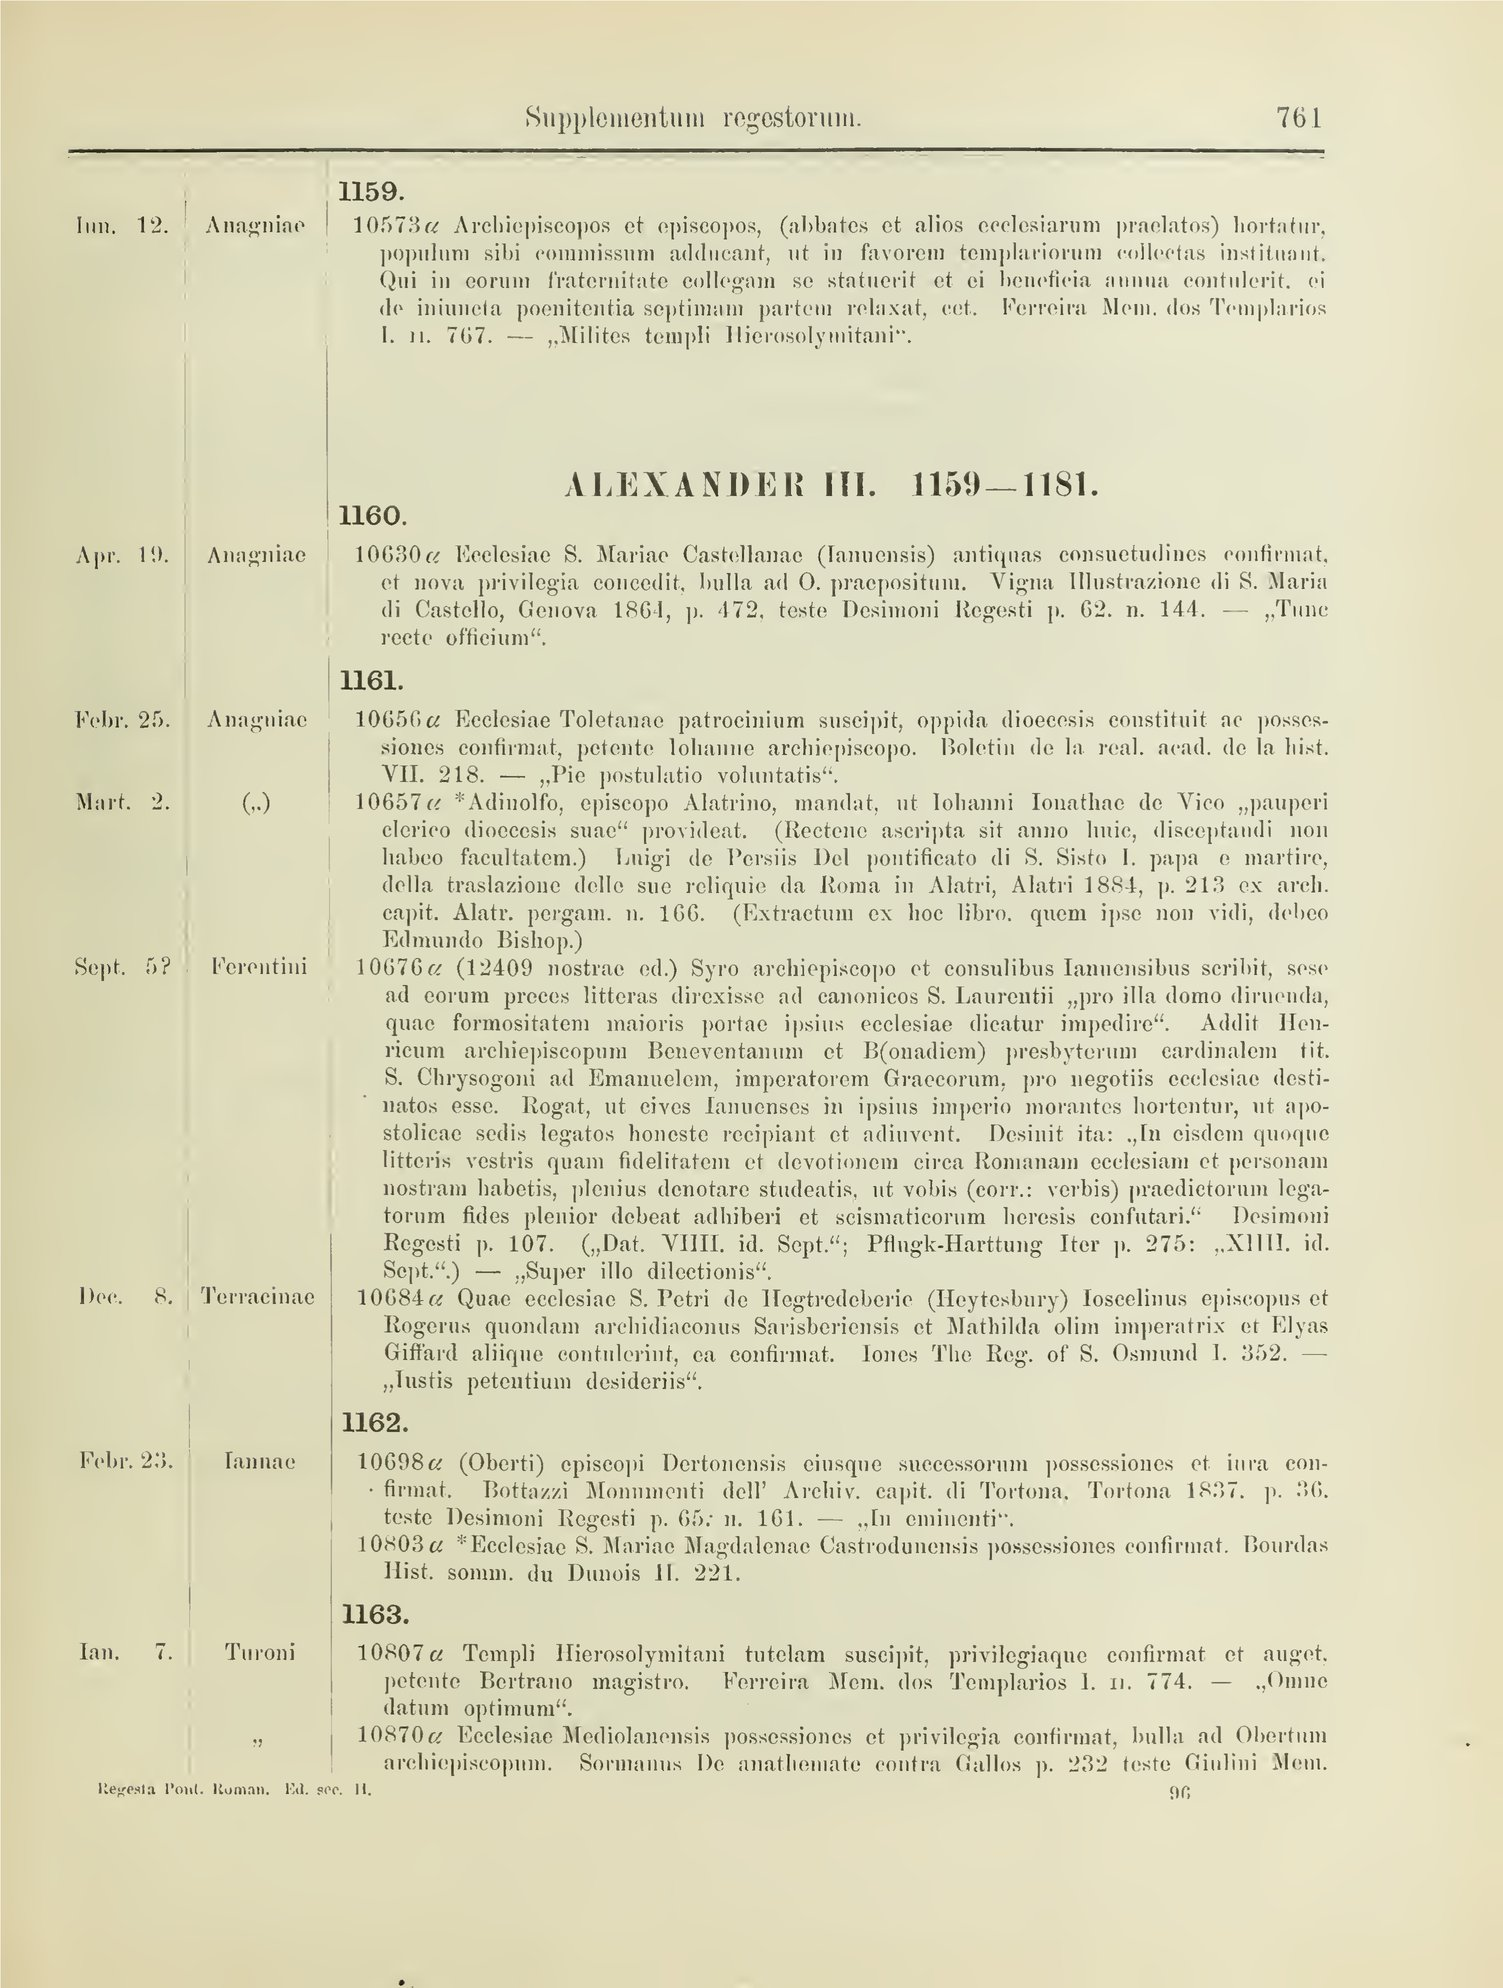
\includegraphics[width=12cm]{images/jaffe2_00772.jpg}
    %légende
    \caption{Exemple d'une page du \textit{Regesta Pontificum Romanorum}, tiré du site du \textit{Monumenta Germaniae Historica} \url{https://www.mgh.de/de}}
    %label
    \label{fig:Jaffe2}
\end{figure}

Le Jaffé permet aux chercheur.re.s de comprendre rapidement le contenu d'une charte, c'est pourquoi c'est une source précieuse pour ce projet.\\

Le schisme alexandrin est la crise la plus importante du XIIème siècle, entraînant une division profonde entre les partisans d'Alexandre III et ceux de l'empire. Néanmoins, la fin de ce schisme s'est accompagnée d'une unification de l'Europe Occidental sous l'égide de l'Eglise.\\ 
On comprend la complexité de ce projet à travers le contexte historique étudié et les différents types de documents et de témoins à intégrer afin de pouvoir potentiellement répondre aux questions que se posent les chercheurs. 